\section*{III. Methods}
\addcontentsline{toc}{section}{III.\hspace{0.12in}Methods}
\hspace{0.25in}
To collect data from our biosensor we first prepare the flowcell chamber with the correct substrate or liquid that acts as our reference point for measuring changes in optical properties. After the chamber is prepared we then turn on the beam and rotate it until the special angle is reached. 

\begin{wrapfigure}{L}{6cm}
    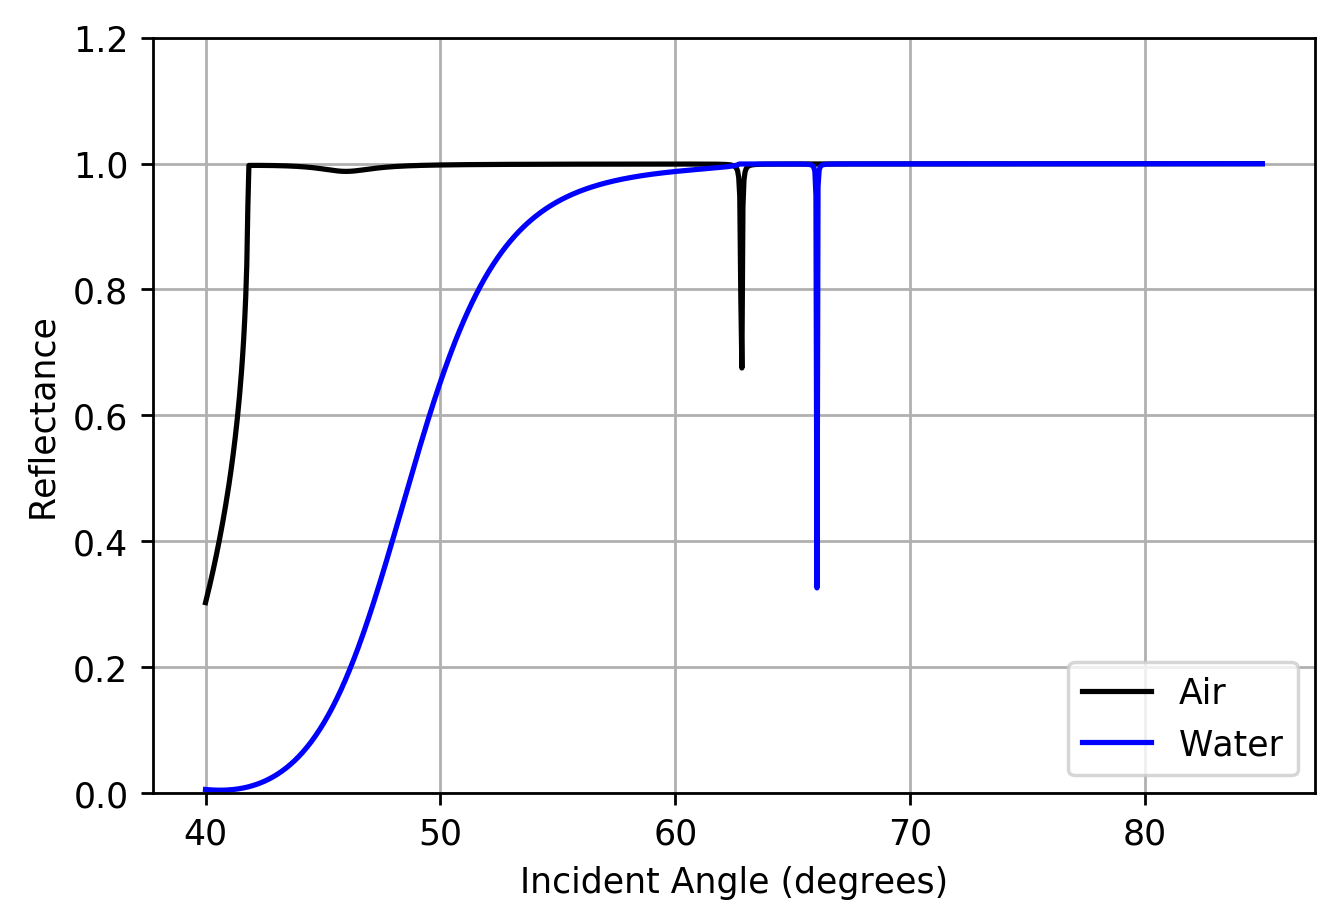
\includegraphics[width=6cm]{reflectivity_dip.png}
\end{wrapfigure}

This is quite a precise angle so we orient the beam near the the mode $\sim 63^{\circ}$ from the prism's surface normal for a chamber filled with water or air using our multilayer stack as seen in ??. This plot was generated from a Python program that I wrote which use a transfer matrix method to generate reflection and transmission amplitudes for a multilayer stack like the one we use in our experiment. To confirm the light has coupled to the surface mode we check the reflected image of the beam for a dark vertical band as seen in ??.

\begin{wrapfigure}{R}{6cm}
	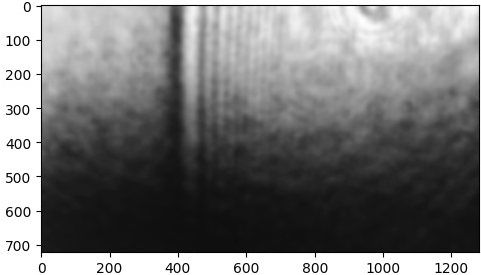
\includegraphics[width=6cm]{darkband.png}
\end{wrapfigure}

As the index of refraction inside the flowcell chamber changes the dark band will translate left or right in our reflected image, depending on whether the index is increasing or decreasing. The shift in location of the band, in pixels, corresponds to an angular shift in the part of the reflected beam giving rise to the dark band. This is shown clearly in ?? as we see that a change from an index of 1.00 (air) to 1.33 (water) corresponds to an angular shift  of about $3^\circ$.


To test our sensor, we first fill the flowcell with water and then inject different concentrations watered down ethanol, isopropal alcohol, and acetone. The table below lists the indices of refraction for all of these liquids.
\begin{center}
\begin{tabular}{| c | c c c c c |}
	\hline
    {}      			& Ethanol & Isopropal Alcohol & Acetone & Water \\
	\hline
	Index of Refraction & 1.361   & 1.3772            & 1.3588  & 1.333 \\
    \hline
\end{tabular}
\end{center}
